\documentclass[10pt]{article}

\usepackage[margin=1in]{geometry} 
\usepackage{amsmath,amsthm,amssymb,bbm,subfig,graphicx,float,physics,listings,fontspec,color}
\usepackage{tikz}
\newfontfamily\Consolas{Consolas}
\definecolor{grey}{rgb}{0.9,0.9,0.9}
\lstset{basicstyle=\ttfamily, breaklines=true, numbers=left, numberstyle=\ttfamily, backgroundcolor=\color{grey}\ttfamily, keywordstyle=\color{blue}\ttfamily, stringstyle=\color{red}\ttfamily, commentstyle=\color{green}\ttfamily}
\DeclareMathOperator*{\argmin}{arg\,min}
\DeclareMathOperator*{\argmax}{arg\,max}
\DeclareMathOperator*{\Conv}{\mathop{\scalebox{1.5}{\raisebox{-0.2ex}{$\ast$}}}}
\DeclareMathOperator*{\vari}{var}

\begin{document}


% --------------------------------------------------------------
%                         Start here
% --------------------------------------------------------------
 
%\renewcommand{\qedsymbol}{\filledbox}
 
\title{\textbf{Report on Project 2}}%replace X with the appropriate number
\author{Zhunxuan Wang, 13300180086\\ %replace with your name
School of Mathematical Sciences} %if necessary, replace with your course title

\maketitle
\section{Convolutional Neural Network}
\subsection{Model Description}
We decided to apply the classic convolutional neural structure \cite{krizhevsky2012imagenet} (shown below) on \texttt{MNIST} dataset
\begin{figure}[H]
\centering
\includegraphics[scale=.9]{convnet.eps}
\caption{The CNN Structure on \texttt{MNIST}}
\label{fig1}
\end{figure}
where the input matrix is the input image (size: $28\times28$), and the output vector is the prediction $10$-D vector. There are two convolution-pooling layers ($32$ and $64$ neurons respectively) at the beginning of the structure. After that, the $7\times7$ feature maps are flattened to vectors. And then it comes a fully connected layer (from $7\times7\times64$ to $1024$) with dropout. The last layer is another fully connected layer (from $1024$ to $10$) which provides the prediction vector.\par
The convolutional and the max-pooling layers will be discussed in detail in next subsections. Obtaining the prediction vector, we take the cross-entropy as the loss function
$$L\left(\mathbf{Y}, \hat{\mathbf{Y}}\right) = -\frac1N\sum\limits_{n \in N}\sum\limits_{i = 1}^{10}Y_{n,i}\log\hat{Y}_{n,i}\text{.}$$\par
Applying the backpropagation \cite{rumelhart1988learning} on the loss function by \texttt{AdamOptimizer} in \texttt{tensorflow}, an iteration of the training process is performed.
\subsection{Convolutional Layer}
The convolutional layer is the core building block of a convolutional network that does most of the computational heavy lifting.\par
First, we introduce the $2$-D convolution
$$\mathbf{B} = \mathbf{A}\Conv\mathbf{K}$$
where $\mathbf{A}$ is the original matrix, $\mathbf{K}$ is the kernel (point spread function) and $\mathbf{B}$ is the convolution result where
$$B_{i,j} = \sum\limits_{u = 1}^m\sum\limits_{v = 1}^nK_{u, v}\cdot A_{i+m-u-c_1+1,j+n-v-c_2+1}$$
where $m$ and $n$ are the size of the kernel $\mathbf{K}$, $c_1$ and $c_2$ are the defined center coordinates of the kernel (generally the center coordinates are the center point of the kernel, and thus $m$ and $n$ are odd numbers). For keeping the size of $\mathbf{B}$ the same as $\mathbf{A}$, we usually pad zeros around $\mathbf{A}$ before convolution.\par
For a convolutional layer ($m$ inputs and $n$ outputs), we have multiple ($m\times n$) kernel matrices, and the $j$-th output will be
$$\mathbf{O}_{j} = \sum\limits_{i = 1}^m\mathbf{I}_i\Conv\mathbf{K}_{i,j}$$
where $\mathbf{I}_i$ is the $i$-th input and $\mathbf{K}_{i,j}$ is the kernel adopted from the $i$-th input to the $j$-th output.
\subsection{Max-Pooling Layer}
The pooling layer operates independently on every depth slice of the input and resizes it spatially, using the \texttt{MAX} operation in this model. The most common form is a pooling layer with filters of size $2\times2$ applied with a stride of $2$ downsamples every depth slice in the input by $2$ along both width and height, discarding $\frac34$ of the activations \cite{nagi2011max}.
\begin{figure}[H]
\centering
\includegraphics[scale=.4]{maxpool.jpeg}
\caption{An Example of Max-Pooling}
\label{fig2}
\end{figure}
In the example showed above, the size of the filter is $2\times2$ and the stride is $2$, and mathematically, the output matrix $\mathbf{O}$ of max-pooling layer is subject to
$$O_{i,j} = \max_{k,l\in\{1,2\}}\left(\mathbf{I}_{i,j}\right)_{k,l}$$
where $\mathbf{I}_{i,j}$ is the submatrix (a $2\times2$ block in the example) at coordinates $\left(i,j\right)$
\subsection{Implementation by \texttt{tensorflow}}
We take the softmax cross entropy as the loss function, setting the max epochs to $2000$, the learning rate to $10^{-4}$, and the batch size to $100$, using the adam optimizer, we have the running result as the picture shows below
\begin{figure}[H]
\centering
\begin{minipage}[b]{0.45\textwidth}
\centering
\includegraphics[scale=1.]{fig1.png}
\label{fig3}
\end{minipage}
\
\begin{minipage}[b]{0.45\textwidth}
\centering
\includegraphics[scale=1.]{fig2.png}
\label{fig4}
\end{minipage}
\caption{The Screenshots of Running Result}
\end{figure}
And we have the accuracy and loss plot against epochs of training and testing process
\begin{figure}[H]
\centering
\begin{minipage}[b]{0.45\textwidth}
\centering
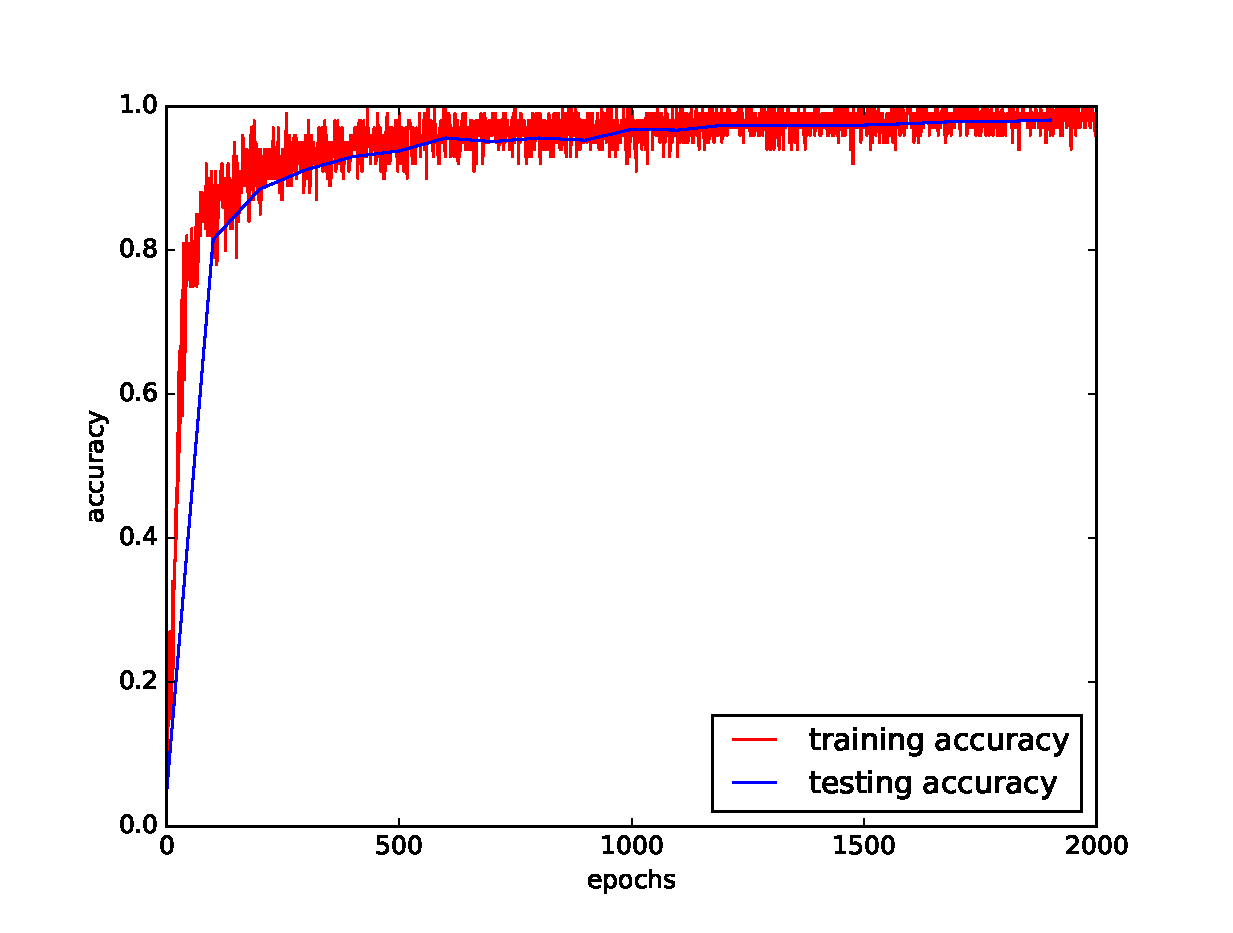
\includegraphics[scale=.37]{plot1.eps}
\label{fig5}
\caption{The Accuracy Plot against Epochs}
\end{minipage}
\
\begin{minipage}[b]{0.45\textwidth}
\centering
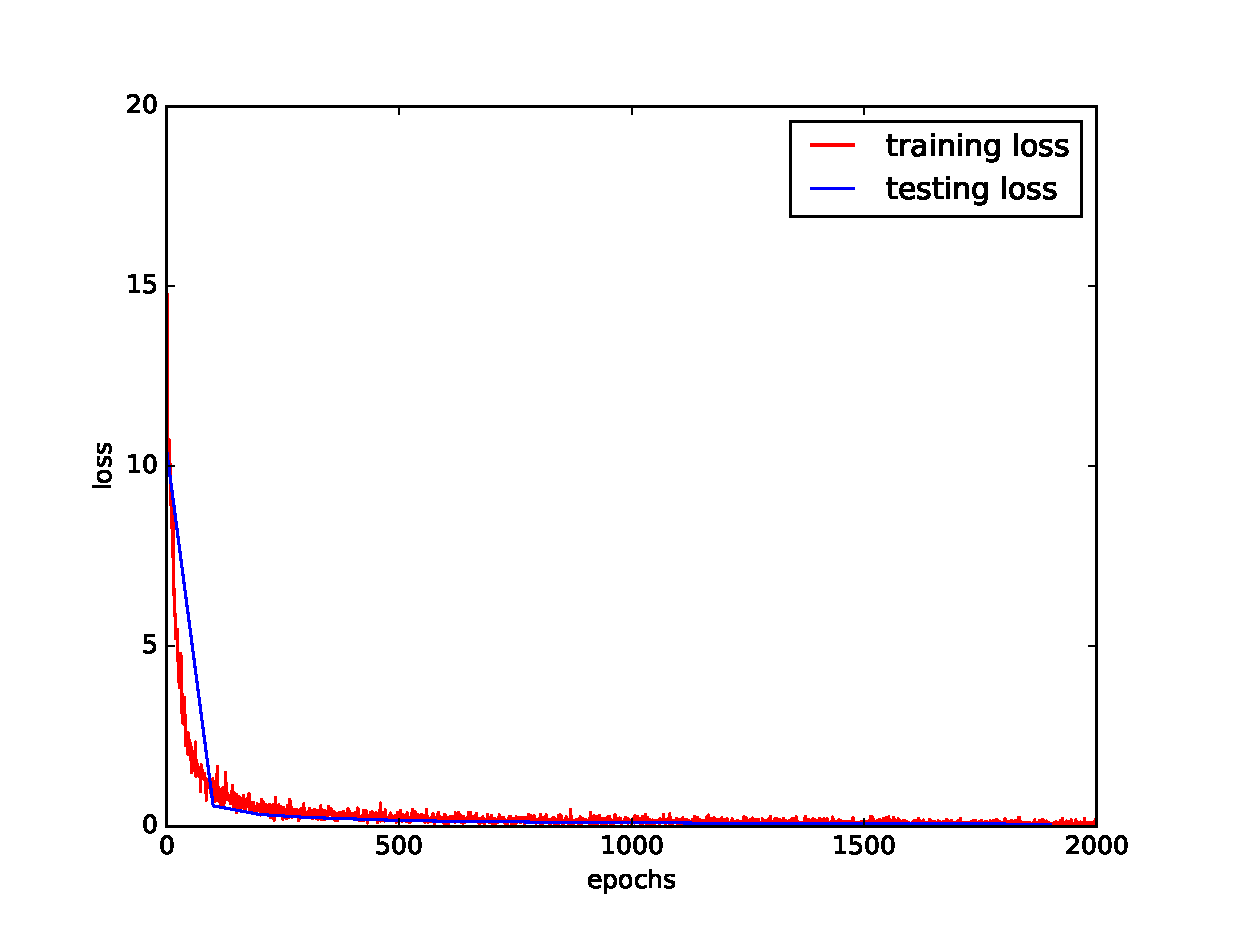
\includegraphics[scale=.37]{plot2.eps}
\label{fig6}
\caption{The Loss Plot against Epochs}
\end{minipage}
\end{figure}
As we observe from the running result picture and the plots, the convergence speed is extremely fast when the number epochs is less than around $100$. This model shows a steady convergence state as the number of epochs reaches around $1200$. The final testing accuracy is $0.981$, of which the cross entropy loss is $0.061292458$.\par
As we infer from the result above, this model's capability is much stronger than the fully connected model that the accuracy of CNN is approximately $8$ percentage higher than FC. And it reached the convergent state without overfitting.
\section{Conclusion}
The classic CNN model showed a great performance on \texttt{MNIST}, which considerably improved the accuracy compared to the fully connected network we experimented on before. It showed a fast convergent trend (accuracy around $0.98$) with the training processes pass, and it was not overfitting.
\clearpage
\bibliographystyle{plain}
\bibliography{ref}
\end{document}